\documentclass[mathserif]{beamer}
\usepackage{natbib}
\usepackage{bibentry}
\usepackage{epstopdf}
\begin{document}
\nobibliography*
\title{Data Assimilation and Herd Dynamics Modeling \\ ENCE689E --- Course Project}
\author{David Prentiss \\ University of Maryland College Park}

\frame{\titlepage}

\begin{frame}
  \frametitle{Agenda}
  \tableofcontents
\end{frame}

\section{Food Security and Pastoral Livelihoods}

\begin{frame}
  \frametitle{Herd Dynamics Modeling}
  \tableofcontents[currentsection]
\end{frame}

\begin{frame}
  \frametitle{\insertsection}
  \begin{itemize}
    \item \emph{Food security} is a measure of food \emph{availability} and \emph{access}.
    \item To be food secure, someone must \emph{produce} food and one must be able to \emph{acquire} and \emph{use} it.
    \item Food security monitoring agencies often focus on the health of \emph{regional livelihoods} to assess regional food security.
    \item A \emph{herd dynamics model} is a component of food security analysis for \emph{pastoral} livelihoods.
  \end{itemize}
\end{frame}

\begin{frame}
  \begin{figure}
    \begin{center}
      \frametitle{\insertsection}
      \includegraphics[width=1\textwidth]{image}

      Photo Credit: Kelley Lynch
    \end{center}
  \end{figure}
\end{frame}

\section{Herd Dynamics Model}

\begin{frame}
  \frametitle{Herd Dynamics Modeling}
  \tableofcontents[currentsection]
\end{frame}

\begin{frame}
  \begin{center}
    \frametitle{\insertsection}
    \begin{itemize}
      \item A Four--state, linear model represents the demographics of a typical herd.
        \begin{itemize}
          \item Adult females die or are sold.
          \item Newborns die or graduate.
          \item Young females die, graduate, or are sold.
          \item Young males die or are sold.
        \end{itemize}
      \item States change each season based on empirical relationships with rainfall--based forcing. They are
        \begin{itemize}
          \item conceptions,
          \item sales,
          \item and mortality.
        \end{itemize}
      \item Rainfall estimates are indexed by quantity and timing.
    \end{itemize}
  \end{center}
\end{frame}

\subsection{Forcing Relationships}
\begin{frame}
  \begin{center}
    \frametitle{\insertsubsection}
    \includegraphics[width=0.9\textwidth]{conceptions}
  \end{center}
\end{frame}

\begin{frame}
  \begin{center}
    \frametitle{\insertsubsection}
    \includegraphics[width=0.9\textwidth]{salefem}
  \end{center}
\end{frame}

\begin{frame}
  \begin{center}
    \frametitle{\insertsubsection}
    \includegraphics[width=0.9\textwidth]{salemale}
  \end{center}
\end{frame}

\begin{frame}
  \begin{center}
    \frametitle{\insertsubsection}
    \includegraphics[width=0.9\textwidth]{mortMat}
  \end{center}
\end{frame}

\begin{frame}
  \begin{center}
    \frametitle{\insertsubsection}
    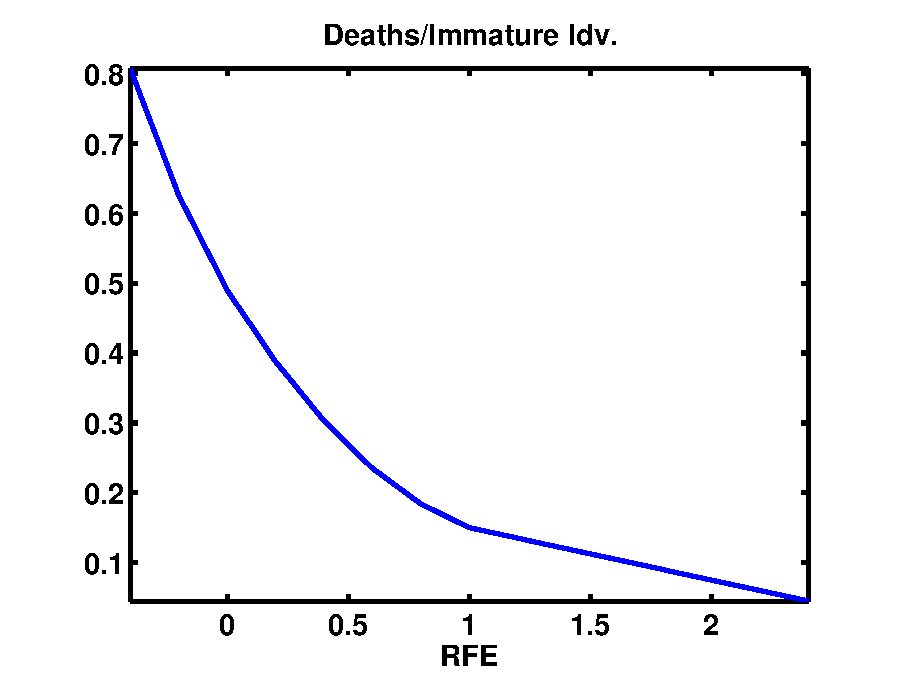
\includegraphics[width=0.9\textwidth]{mortImm}
  \end{center}
\end{frame}

\subsection{Formulation and Error}
\begin{frame}
  \begin{center}
    \frametitle{\insertsubsection}
    \begin{align}
      y_{\text{AF}}^{t+1} &= [y_{\text{AF}}^t + y_{\text{YF}}^t - f_{\text{SF}}^ty_{\text{AF}}^t - f_{\text{MM}}^ty_{\text{AF}}^t]w_{\text{AF}}\\
      y_{\text{NB}}^{t+1} &= [f_{\text{C}}^ty_{\text{AF}}^t]w_{\text{NB}}\\
      y_{\text{YF}}^{t+1} &= [0.5(y_{\text{NB}}^t - f_{\text{MI}}^ty_{\text{NB}}^t) - f_{\text{MM}}^ty_{\text{YF}}^t]w_{\text{YF}}\\
      y_{\text{YM}}^{t+1} &= [y_{\text{YM}}^t + y_{\text{NB}}^t - y_{\text{YF}}^{t+1} - f_{\text{SM}}^ty_{\text{YM}}^t - f_{\text{MM}}^ty_{\text{YM}}^t]w_{\text{YM}}
    \end{align}
  \end{center}
  \begin{itemize}
    \item $y$ are model states.
    \item $f$ are rainfall dependent rates of change.
    \item $w$ are multiplicative model error.
    \item $w\sim\ln\mathcal{N}(\mu,\sigma)$, $\bar{w}=1$, $\sigma_w^2 = 0.001$.
    \item Multiplicative, lognormal error avoids negative values.
    \item It also means we cannot use the KF.
  \end{itemize}
\end{frame}

\section{General Characteristics}

\begin{frame}
  \frametitle{Herd Dynamics Modeling}
  \tableofcontents[currentsection]
\end{frame}

\begin{frame}
  \begin{center}
    \frametitle{\insertsection}
    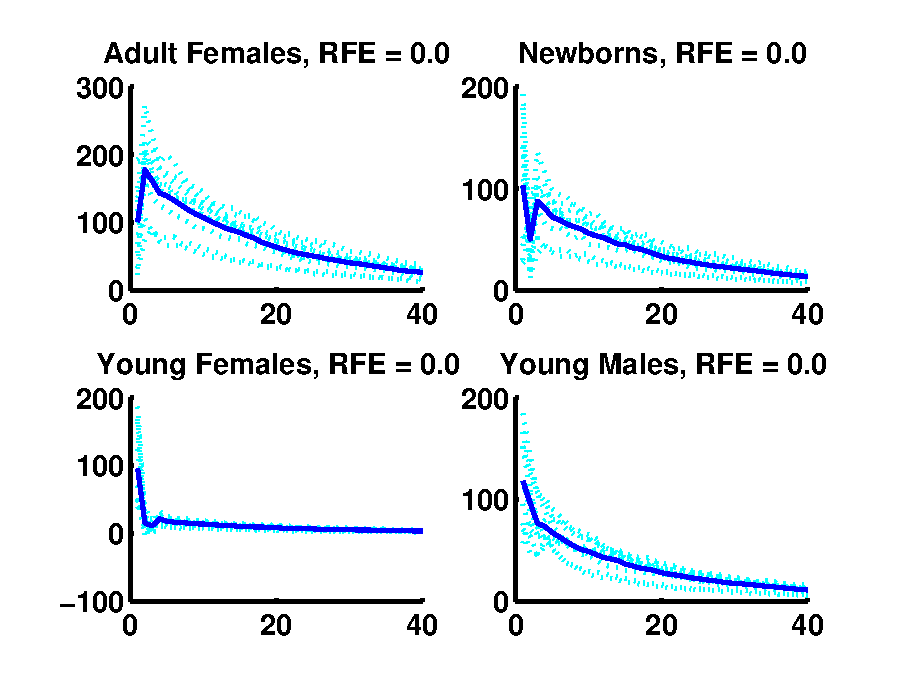
\includegraphics[width=0.9\textwidth]{general0}
  \end{center}
\end{frame}

\begin{frame}
  \begin{center}
    \frametitle{\insertsection}
    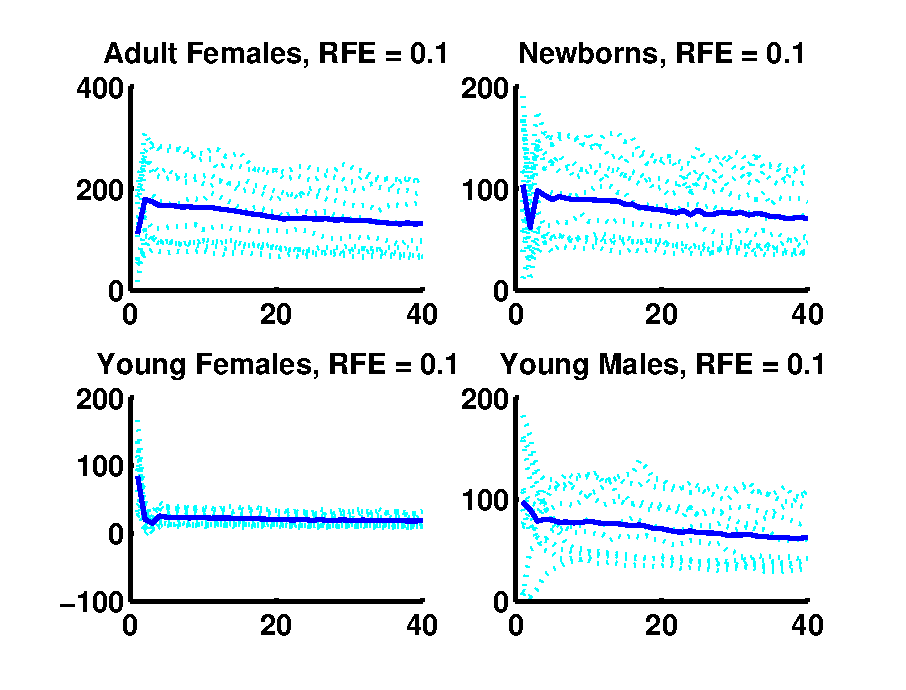
\includegraphics[width=0.9\textwidth]{general1}
  \end{center}
\end{frame}

\begin{frame}
  \begin{center}
    \frametitle{\insertsection}
    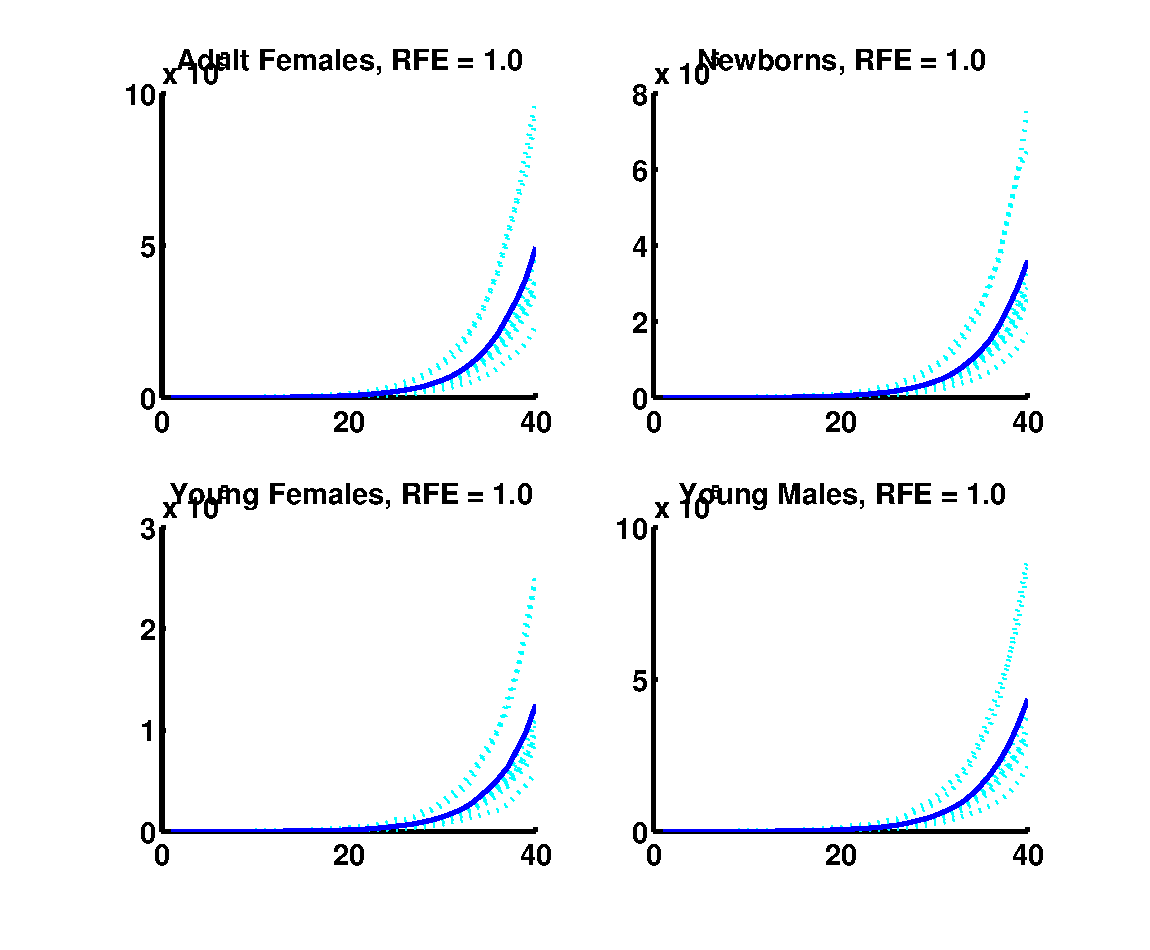
\includegraphics[width=0.9\textwidth]{general10}
  \end{center}
\end{frame}

\begin{frame}
  \begin{center}
    \frametitle{\insertsection}
    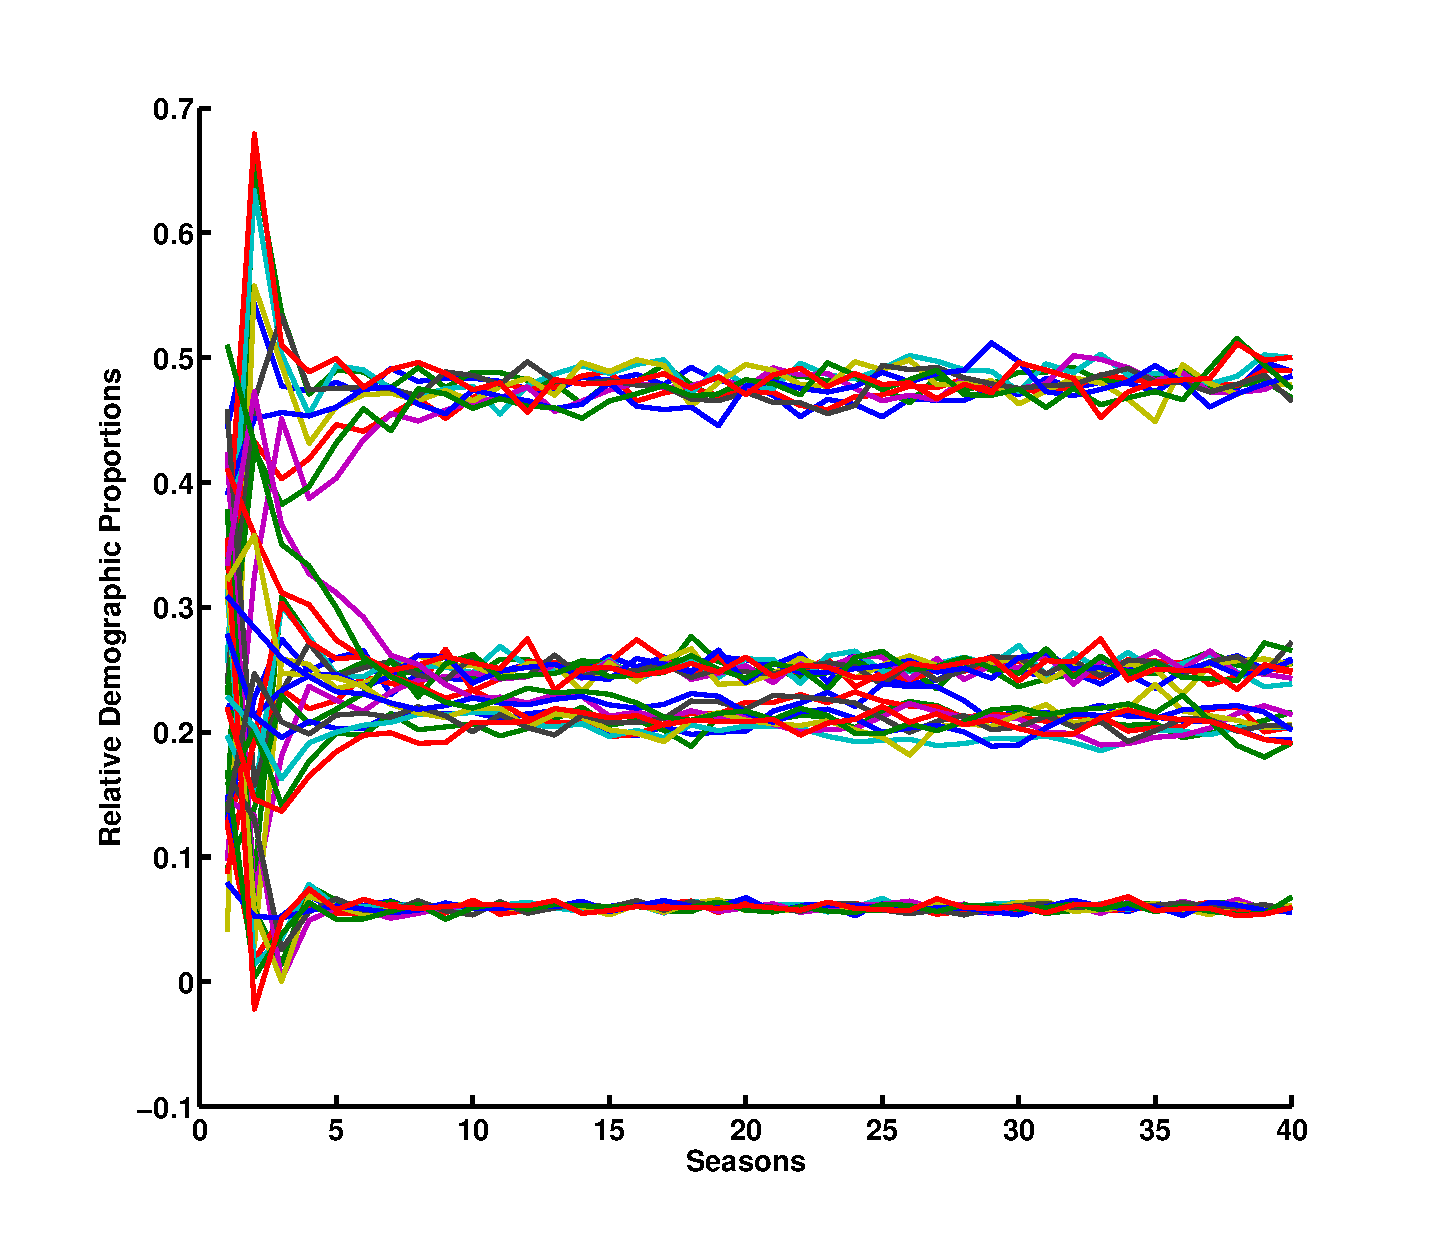
\includegraphics[width=0.9\textwidth]{relprop}
  \end{center}
\end{frame}

\section{Data Assimilation}

\begin{frame}
  \frametitle{Herd Dynamics Modeling}
  \tableofcontents[currentsection]
\end{frame}

\subsection{Synthetic Truth}
\begin{frame}
  \begin{center}
    \frametitle{\insertsubsection}
    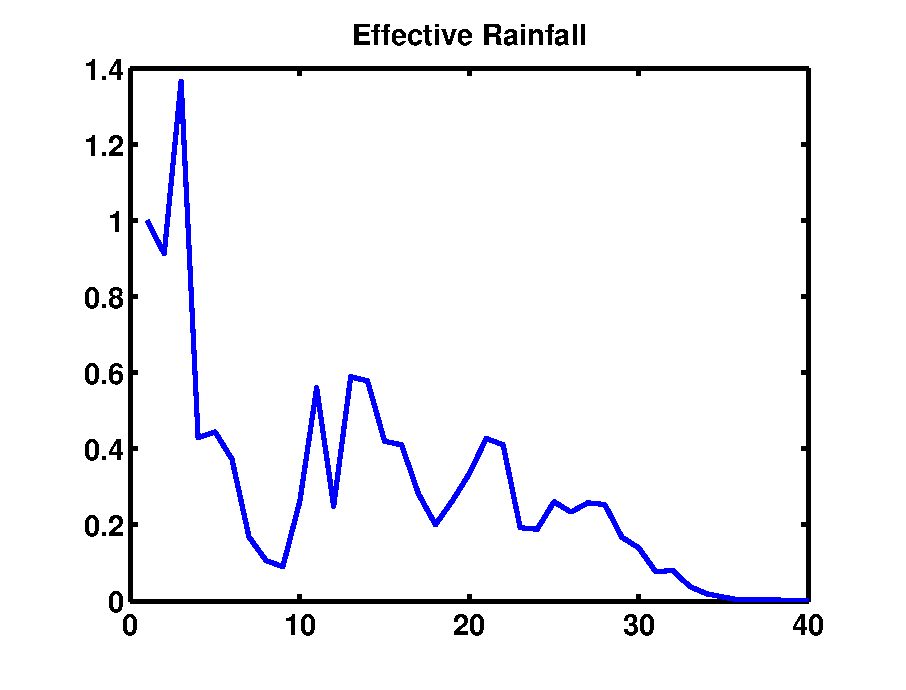
\includegraphics[width=0.9\textwidth]{forcing}
  \end{center}
\end{frame}

\begin{frame}
  \begin{center}
    \frametitle{\insertsubsection}
    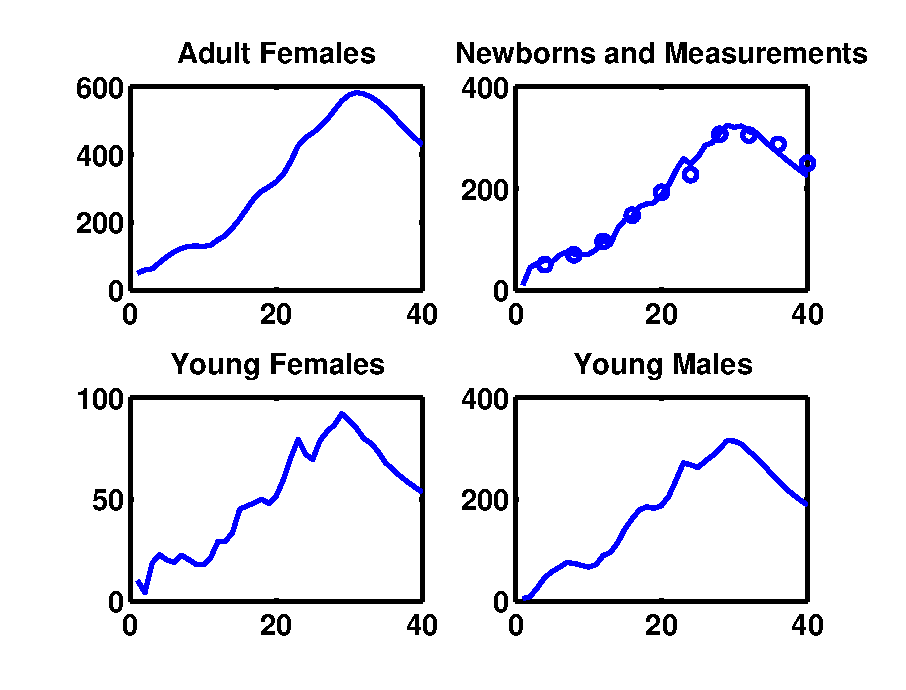
\includegraphics[width=1\textwidth]{truth}
  \end{center}
\end{frame}

\subsection{Initial Conditions}

\begin{frame}
  \begin{center}
    \frametitle{\insertsubsection}
    \begin{itemize}
      \item True initial conditions: $(50\ 10\ 10\ 5)^T$
      \item Ensemble initial conditions: $y_0\sim\mathcal{U}(0,200)$, uncorrelated
      \item 100--member ensemble initial mean: $(95\ 94\ 101\ 98)^T$
      \item 100--member ensemble initial covariance:

      $\left(\begin{array}{cccc} 3345.0 & -515.0 & 220.6 & -144.6\\ -515.0 & 2995.0 & -665.7 & -53.02\\ 220.6 & -665.7 & 3431.0 & 72.85\\ -144.6 & -53.02 & 72.85 & 3061.0 \end{array}\right)$
    \end{itemize}
  \end{center}
\end{frame}

\begin{frame}
  \begin{center}
    \frametitle{\insertsubsection}
    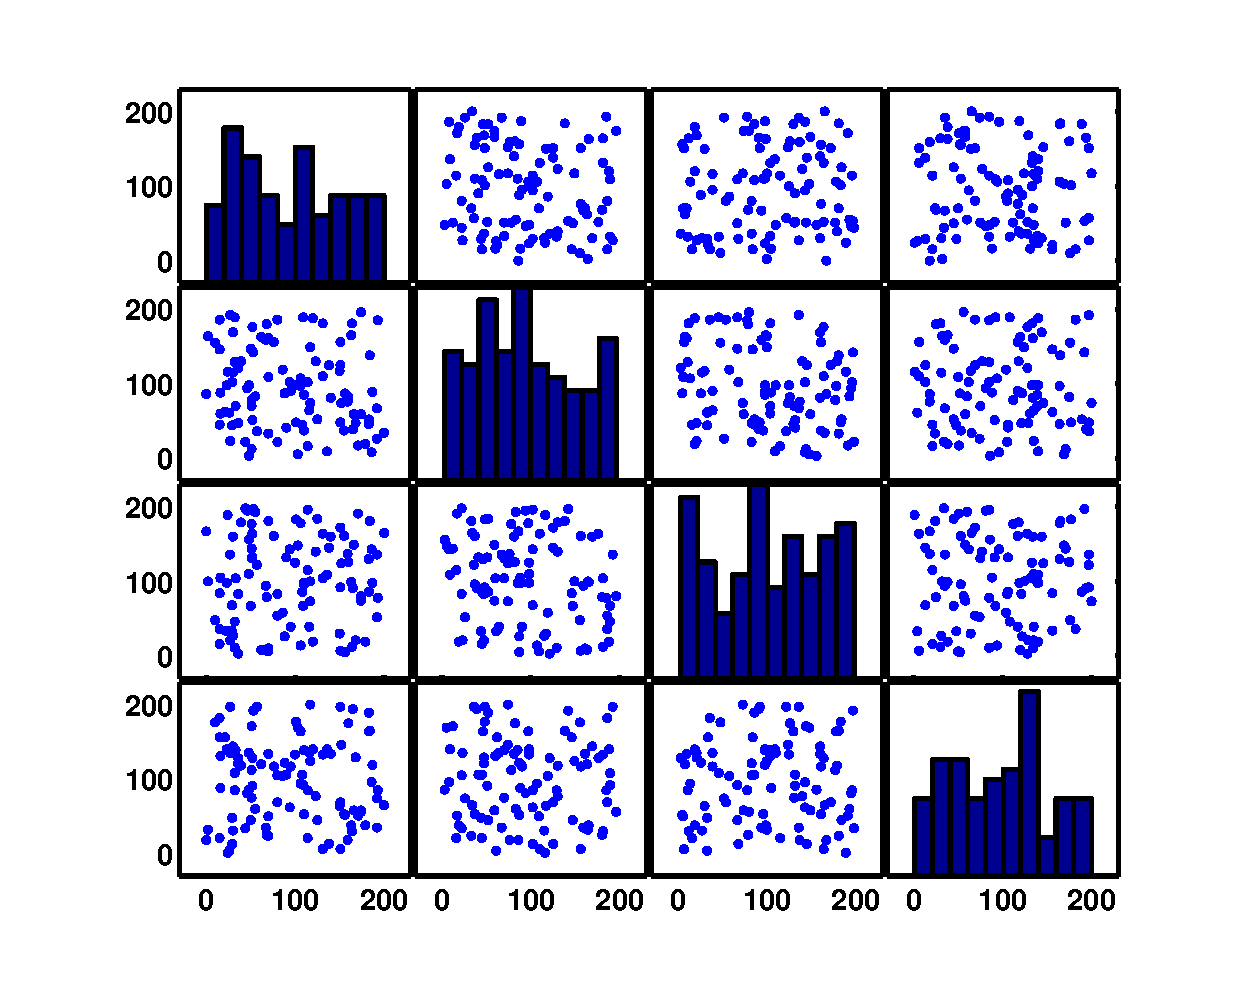
\includegraphics[width=1\textwidth]{initcov}
  \end{center}
\end{frame}

\begin{frame}
  \frametitle{Open Loop}
  \begin{center}
    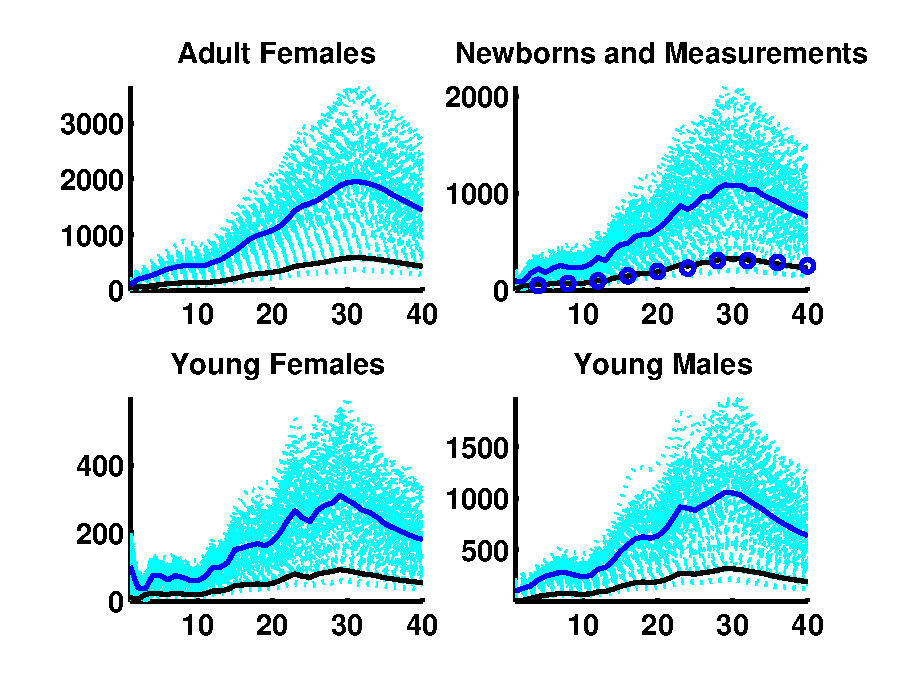
\includegraphics[width=1\textwidth]{openloop}
  \end{center}
\end{frame}

\begin{frame}
  \begin{center}
    \frametitle{Ensemble Kalman Filter}
    t = 30
    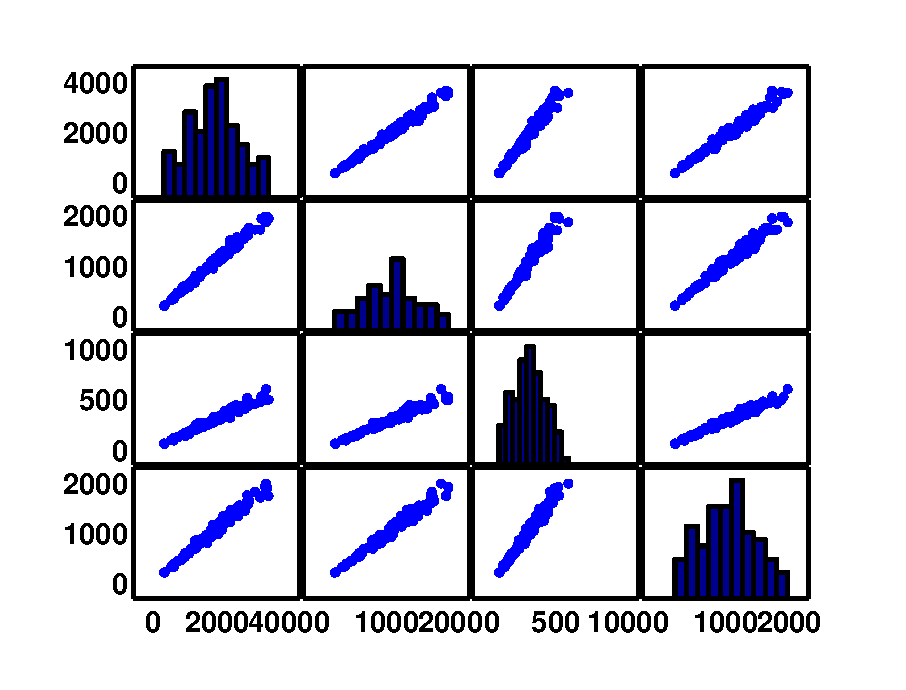
\includegraphics[width=1\textwidth]{ol30cov}
  \end{center}
\end{frame}

\begin{frame}
  \begin{center}
    \frametitle{Ensemble Kalman Filter}
    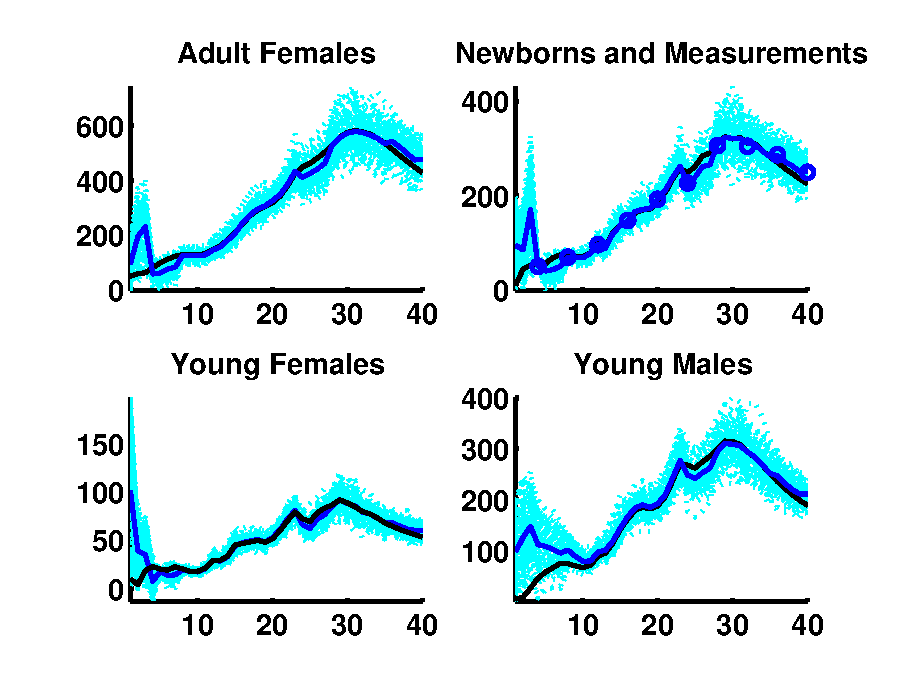
\includegraphics[width=1\textwidth]{filtered}
  \end{center}
\end{frame}

\begin{frame}
  \begin{center}
    \frametitle{Ensemble Kalman Filter}
    t = 30
    \includegraphics[width=1\textwidth]{kf30cov}
  \end{center}
\end{frame}

\begin{frame}
  \begin{center}
    \frametitle{Ensemble Kalman Filter}
    \begin{table}
      \begin{tabular}{rrr}
        & Bias & RMSE \\
        \hline
        Open loop & 441.2 & 565.2 \\
        EnKF & 6.5 & 31.1
      \end{tabular}
      \caption{Skill of open loop vs. EnKF}
    \end{table}
  \end{center}
\end{frame}

\subsection{Ensemble Size}

\begin{frame}
  \begin{center}
    \frametitle{Ensemble Kalman Filter}
    \begin{table}
      \begin{tabular}{rrrr}
        Ensemble members & 10 & 100 & 1000 \\
        \hline
        Bias & 10.5 & 6.5 & 6.5 \\
        RMSE & 36.3 & 31.1 & 31.7
      \end{tabular}
      \caption{Skill for various ensemble sizes}
    \end{table}
  \end{center}
\end{frame}

\subsection{Model Error Variance}

\begin{frame}
  \begin{center}
    \frametitle{Ensemble Kalman Filter}
    \begin{table}
      \begin{tabular}{rrrr}
        Model Error Variance & 0.001 & 0.01 & 0.1 \\
        \hline
        Bias & 6.5 & 7.2 & 9.7\\
        RMSE & 31.1 & 30.9 & 40.7
      \end{tabular}
      \caption{Skill for various model error variances}
    \end{table}
  \end{center}
\end{frame}

%\bibliographystyle{plainnat}
%\bibliography{project}
\end{document}
